\section{Platinenaufbau}
Die Platine ist mit mehreren Bauteilen ausgestattet, die bis auf drei selbst zu dimensionierende Widerstände bereits vollständig bestückt ist.

Zur Erklärung von Abbildung 4.1 hier eine kurze Information zu den wichtigsten Abkürzungen:
\begin{itemize}
    \item R: Widerstand
    \item C: Kondensator
    \item J: Stecker/Relais
\end{itemize}

Die wichtigsten Bauteile sind:
\begin{itemize}
    \item J1: Anschluss an den FieldFox (Ausgangssignal)
    \item J40: Verbindung zum Oszillator (Taktquelle für die Schaltung) und Anschluss an den FieldFox (Eingangssignal)
    \item R47-49: Widerstände zur Arbeitspunkteinstellung
    \item Oszillator (XLL536C50.000000X): HF-Taktsignal
    \item Transistor (BFR181W)
    \item Operationsverstärker (U20-LMV651MG/NOPB; U21-NCX2200GW,125)
    \item USB-UART-IC (FT232RL)
\end{itemize}

\begin{figure}[h]
    \centering
    \includegraphics[width=1.0\textwidth]{Pictures/Bestückungsplan.jpg}
    \caption{Bestückungsplan}
\end{figure}

\section{Bestückung der PCB}
Die in Kapitel 3 bestimmten Widerstände werden nun im Rahmen der praktischen Umsetzung der Schaltung auf die bereits vorbereitete Platine angebracht. Auf dem Bestückungsplan entspricht R47 dem Widerstand R3 mit 1000~Ohm, R48 dem Widerstand R4 mit 4700~Ohm und R49 dem Widerstand R5 mit 330~Ohm. Beim Löten der drei Widerstände wird auf eine saubere und präzise Löttechnik geachtet, um die gewünschte elektrische, mechanische und HF-technische Funktion der Schaltung zu garantieren.
\begin{figure}[h]
    \centering
    \includegraphics[width=0.54\textwidth]{Pictures/Platinebestückt.jpg}
    \caption{Bestückte Platine}
\end{figure}

\section{DC-Pegel verifizieren}
Nach dem Bestücken der Platine wird die Funktionalität der Schaltung überprüft. Hierzu wird eine Versorgungsspannung von 4,8~V angelegt, um die Gleichspannungspegel an den relevanten Punkten der Schaltung zu überprüfen. Die abfallenden Spannungen werden mit einem Oszilloskop gemessen. Relevant sind die Spannungsabfälle über R47, R48 und R49. Diese gemessenen Spannungen werden mit den idealen Werten der Simulation verglichen.
\clearpage
\section{SOLT-Kalibrierung}
Das Ziel der SOLT-Kalibrierung (Short, Open, Load, Through) ist die Eliminierung von systematischen Messfehlern, die durch die Messeinrichtung (Kabel, Adapter etc.) selbst entstehen und die Messung verfälschen.
Durch das Messen dieser Fehler lässt sich die Messung korrigieren.
Dafür werden vier verschiedene Kalibrierstandards benötigt:
\begin{itemize}
    \item Short (Kurzschluss): Ein Kurzschluss-Standard wird an den Messport des VNAs angeschlossen. Da ein idealer Kurzschluss alle Leistung reflektiert und eine Phasenverschiebung von 180 Grad verursacht, misst der VNA diese Referenz. Abweichungen vom Ideal werden erfasst.
    \item Open (Leerlauf): Ein Leerlauf-Standard wird angeschlossen. Ein idealer Leerlauf reflektiert ebenfalls die gesamte Leistung, jedoch mit einer Phasenverschiebung von 0 Grad. Auch hier werden Abweichungen aufgezeichnet.
    \item Load (Abschluss/Last): Ein Präzisions-Abschlusswiderstand (meist 50~Ohm) wird angeschlossen. Ein idealer Abschlusswiderstand absorbiert die gesamte Leistung ohne Reflexion. Dies dient dazu, die Leistungsanpassung des Systems zu kalibrieren.
    \item Through (Durchgang): Bei einer 2-Port-Messung wird ein direkter Durchgang (ein kurzes, bekanntes Kabel oder ein Adapter) zwischen den beiden Messports des VNAs angeschlossen. Dies ermöglicht die Kalibrierung der Übertragungseigenschaften zwischen den Ports und die Korrektur von Phasen- und Amplitudenfehlern des Übertragungspfades.
\end{itemize}
\begin{figure}[h]
    \centering
    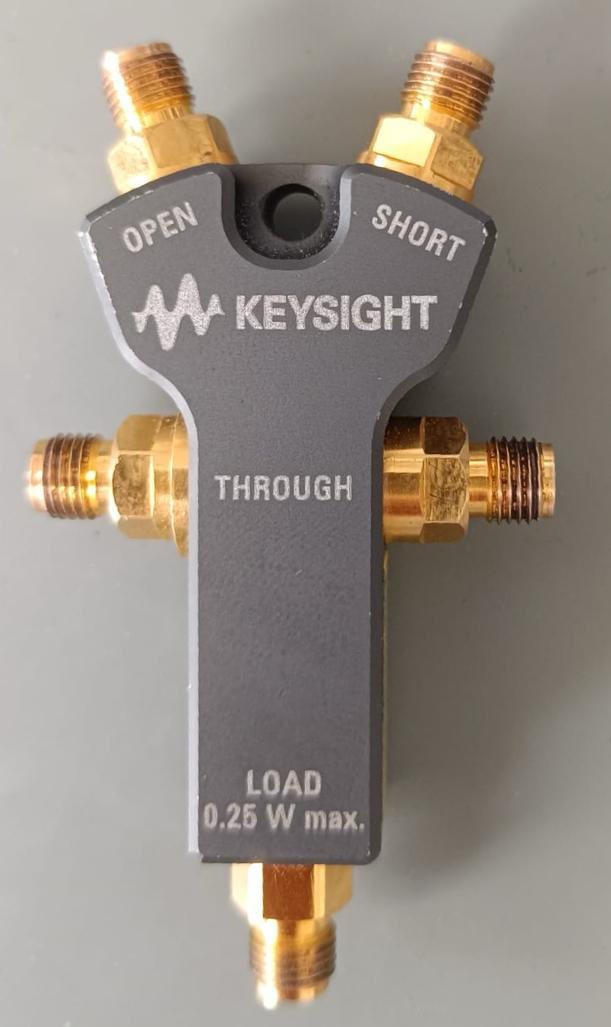
\includegraphics[width=0.25\textwidth]{Pictures/Keysightkallibrierung.jpg}
    \caption{Kalibrierung am Keysight FieldFox}
\end{figure}
\clearpage

Die Kalibrierung wird am Keysight FieldFox durchgeführt. Sie erfolgt über sieben Schritte, die vom Gerät angeleitet werden. Danach ist das Gerät bereit für die Messung.
\subsection{Verfizierung der Qualität der SOLT-Kalibrierung}
Unter Beibehaltung des Messaufbaus werden nun die S-Parameter, der bei der Kalibrierung verwendeten Kabel, betrachtet. Ist die Kalibrierung gelungen sollte unter optimalen Bedingungen bei den Streuparametern keine Dämpfung mehr angezeigt werden, da die Kalibrierung die Kabeldämpfung herausrechnet. In unserem Fall ist die zeigt die Messung eine kleine Abweichung, ist jedoch sehr nahe am Optimum. Es ist daher keine erneute Kalibrierung von Nöten.


\section{Vergleich zur Simulation}
Die Simulation wurde, wie zuvor beschrieben, mit der Software Advanced Design System (ADS) durchgeführt. In der Simulation fällt über R47 eine Spannung von 0,811~V, über R48 eine Spannung von 3,989~V und über R49 eine Spannung von 1,27~V ab. Wir überprüfen nun, ob sich unsere Messung mit den simulierten Werten deckt.

\begin{table}[h]
    \centering
    \begin{tabular}{|l|l|l|}
        \hline
        \textbf{Widerstand} & \textbf{Simulation [V]} & \textbf{Messung [V]} \\
        \hline
        R47 & 0{,}811 & 0{,}809 \\
        \hline
        R48 & 3{,}989 & 3{,}991 \\
        \hline
        R49 & 1{,}27  & 1{,}26 \\
        \hline
    \end{tabular}
    \caption{Vergleich von simulierten und gemessenen Spannungswerten}
\end{table}

\clearpage
